
\vspace{1cm}
{\let\clearpage\relax \chapter{Dataset}}

Il dataset utilizzato è costituito dalla serie storica oraria di misurazioni di CO, in un periodo dal marzo 2004 al febbraio 2005, per un totale di 8526 osservazioni. L’obiettivo è prevedere i 744 valori orari del mese di marzo 2005. 


\begin{figure}[H]
\centering
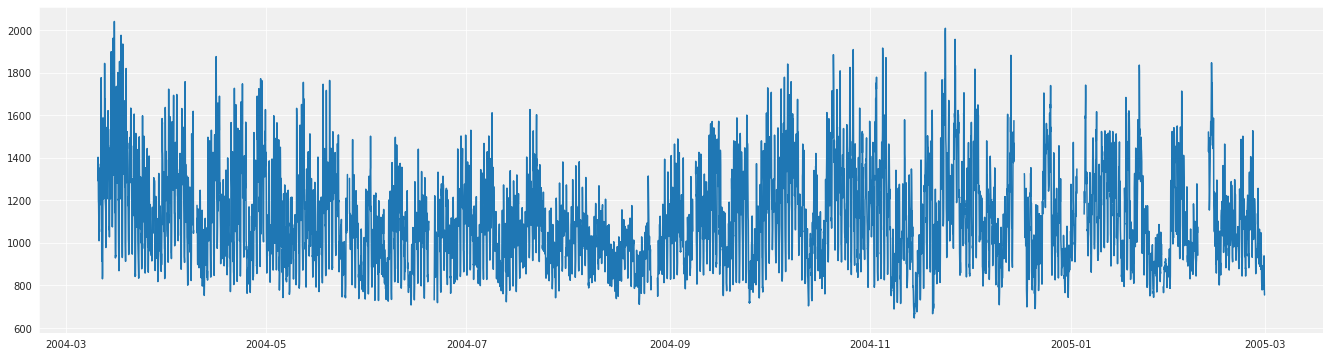
\includegraphics[width=14cm]{Pictures/ts.png}
\caption{Serie storica iniziale}
\end{figure}

Non si nota nessun outlier evidente dovuto ad errori di misurazione, ma, al contempo, la serie presenta 365 missing values. Per far fronte a questo problema, ognuno di esso è stato sostituito dalla media dei 3 valori precedenti alla stessa ora e stesso giorno della settimana. 

Successivamente, il dataset è stato diviso in training set e validation set. Si è scelto di considerare come validation set l'ultimo mese di dati a disposizione in modo da mantenere un buon numero di osservazioni per il training. Questo porta ad un training set di 7854 osservazioni (92.1\%) ed un validation set di 672 osservazioni (7.9\%). 

\begin{figure}[H]
\centering
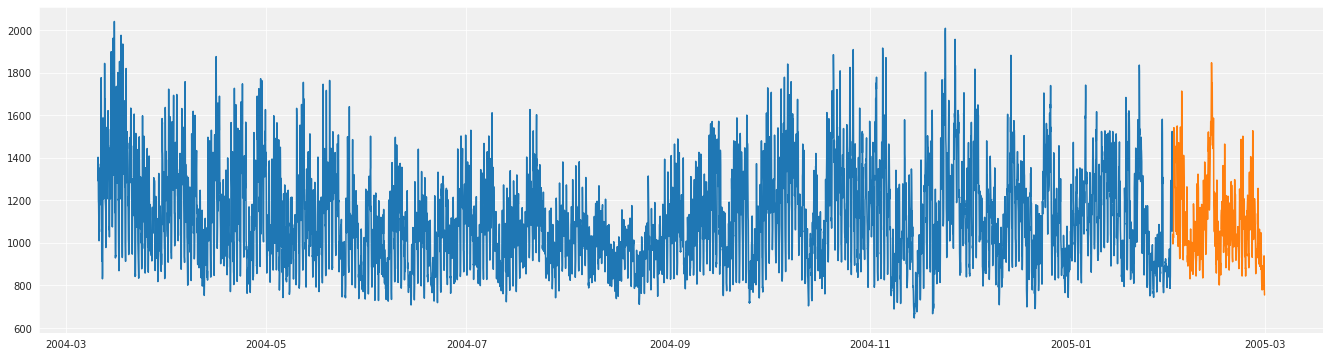
\includegraphics[width=14cm]{Pictures/train_val.png}
\caption{Suddivisione in training set e validation set della serie senza missing values}
\label{train_val}
\end{figure}

Esplorando più a fondo i dati, si può notare la presenza di più stagionalità: da una parte giornaliera, con una rilevazione inferiore di CO nelle ore notturne, mentre dall'altra settimanale, con una rilevazione inferiore nei week end. 

\begin{figure}[H]
\centering
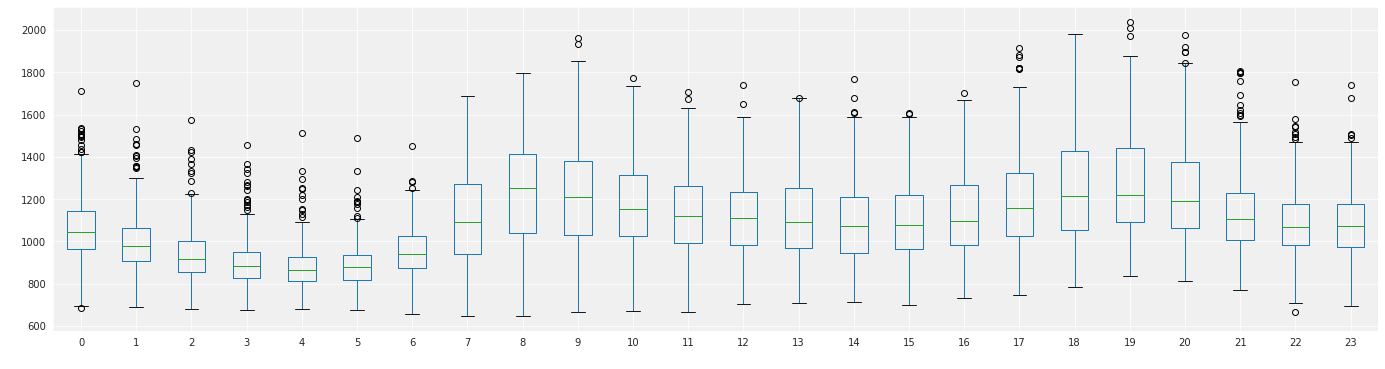
\includegraphics[width=14cm]{Pictures/co_oraria.png}
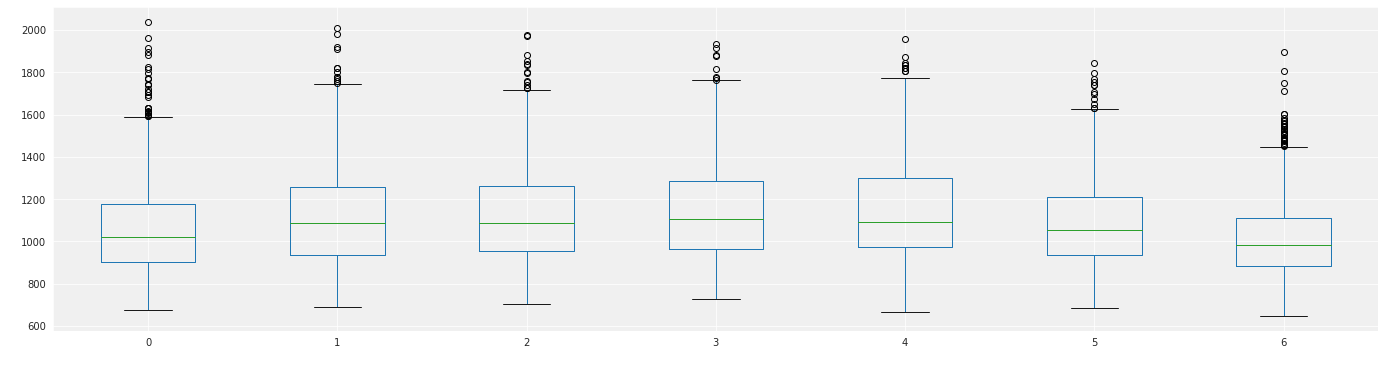
\includegraphics[width=14cm]{Pictures/co_settimanale.png}
\caption{Boxplot che descrivono stagionalità rispettivamente giornaliera e settimanale.}
\end{figure}